\documentclass[11pt]{article}
\usepackage{amsmath,amssymb,amsthm}
\usepackage{fullpage}
\usepackage{amsmath,amssymb,amsthm}
\usepackage{tikz}
\usepackage[hidelinks]{hyperref}

\newtheorem{theorem}{Theorem}[section]
\newtheorem{lemma}[theorem]{Lemma}
\newtheorem{proposition}[theorem]{Proposition}
\theoremstyle{remark}
\newtheorem{remark}[theorem]{Remark}
\newcommand{\kk}{\mathbb K}
\newcommand{\U}{U_q}
\newcommand{\slN}{\mathfrak{sl}_n}
\newcommand{\bp}{\mathfrak b_+}
\newcommand{\bm}{\mathfrak b_-}
\newcommand{\np}{\mathfrak n_+}
\newcommand{\Skein}{\mathcal S_n}
\newcommand{\redS}{\overline{\mathcal S}_n}
\newcommand{\Bstar}{\mathfrak B^*}
\newcommand{\Bigon}{\mathfrak B}
\newcommand{\ot}{\otimes}
\newcommand{\id}{\mathrm{id}}
\newcommand{\la}{\langle}
\newcommand{\ra}{\rangle}
\newcommand{\cD}{\mathcal D}
\newcommand{\Oq}{\mathcal O_q(SL_n)}

\newcommand{\fptitle}{Review of Problem 3 -- ProofCouncil}
\newcommand{\reviewtag}{Reviewer 2}
\usepackage{fp-review}

\begin{document}
\maketitle

\section{Review}
The submission is correct. The argument is similar to one of the other submissions and to the human proof. A presentation for the generalized quantum double $\mathcal{D}$ is established first. The reduced stated skein algebra of the punctured bigon is identified, as a vector space, with $U_q(\mathfrak{b}_-) \otimes U_q(\mathfrak{b}_+)$, the tensor product of the Borel subalgebras of $U_q(\mathfrak{sl}_n)$. This uses an intermediate isomorphism relying on height-exchange relations and a saturated systems of arcs; these arguments are carefully explained. An algebra homomorphism from $\mathcal{D}$ to the reduced stated skein algebra is defined, and it is shown to be an isomorphism by viewing it as a composition of three linear isomorphisms.

The exposition is clear. A helpful overview of the strategy is given in the beginning. This subject is inherently diagrammatic, and including pictures would greatly aid the exposition (this comment applies to all the submissions).  

The attributions seem mostly complete. There is a fairly comprehensive paragraph describing relations to existing literature. The submission appropriately cites work of Korinman, who established the isomorphisms in the problem statement for the case $n=2$. There are abundant precise references throughout the solution which also aid the exposition. 


\paragraph{Correctness.}
\begin{itemize}
	\item  1: essentially flawless mathematical argument
	\item  0.5: minor errors that are easily corrected
	\item  0: blank solution, or acknowledged partial result
	\item  $-0.5$: major errors
	\item  $-1$: proposed proof makes no progress towards the result.
\end{itemize}
Note that points should be docked for wrong statements/ solutions.

\noindent Score: $1$

\paragraph{Exposition.}
\begin{itemize}
	\item  1: well-written and clear solution.
	\item  0: argument that is possible to follow with serious effort
	\item  $-1$: very poor exposition
\end{itemize}

\noindent Score: $1$

\paragraph{Attributions.}
\begin{itemize}
	\item  1: solutions contains fully appropriate attributions
		to related work and theorems being used.
	\item  0: moderate issues with missing attributions or hallucinated references
	\item  $-1$: blatant plagiarism or hallucinations
\end{itemize}

\noindent Score: $1$

\newpage
\section{Submission with inline comments}


\begin{abstract}
We construct an explicit algebra isomorphism between the generalized
quantum double $\cD=\U(\bm)\bowtie\U(\bp)$ of the Borel subalgebras of
the simply-connected $\U(\slN)$, for the Drinfeld--Tanisaki skew
pairing, and the reduced stated $SL_n$-skein algebra $\redS(\Bstar)$ of
a bigon with one interior puncture: the two families of horizontal arcs
of $\Bstar$ become a lower and an upper triangular quantum matrix, whose
diagonal entries generate the two copies of the weight torus and whose
off-diagonal entries are root vectors up to toral factors. We deduce
that $\U(\slN)$ is the quotient of $\redS(\Bstar)$ by the relations
$b_{aa}c_{aa}=1$ between the diagonal entries.
For $n=2$ both statements are due to Korinman. The proof combines the
L\^e--Sikora factorization of stated skein algebras with the
Faddeev--Reshetikhin--Takhtajan realization of quantum Borel algebras
by triangular quantum matrices, with all normalizations made explicit.
\end{abstract}

\section{Introduction}

\subsection{The problem}

Stated skein algebras attach to a surface with marked boundary an
algebra spanned by framed oriented tangles (``webs'') whose endpoints
carry labels called states, modulo local skein relations; they were
introduced for $SL_2$ by L\^e \cite{Le}, developed by Costantino and
L\^e \cite{CL}, and defined for $SL_n$ by L\^e and Sikora \cite{LS}. For the \emph{bigon} $\Bigon$, a closed disk
with two ideal points removed from its boundary, the stated
$SL_n$-skein algebra is the quantum coordinate algebra $\Oq$
\cite[Theorem 6.3]{LS}. The problem treated here concerns the
\emph{punctured bigon} $\Bstar$, obtained from $\Bigon$ by removing one
interior point. It asks:
(1) to construct an explicit algebra isomorphism between
$\redS(\Bstar)$, the reduced stated $SL_n$-skein algebra of $\Bstar$
(Section~\ref{sec:interp}), and the generalized quantum double $\cD=\U(\bm)\bowtie\U(\bp)$ of the
Borel subalgebras of the simply-connected quantum group $\U(\slN)$
(the algebra written $U^{ext}_q(\mathfrak{sl}(n))$ in
\cite[Section 8.5.3]{KS}), the double being taken with respect to the
Drinfeld--Tanisaki skew pairing
\begin{equation}\label{eq:problempairing}
 \la\hat K_i,\hat K_j\ra=q^{\frac1n-\delta_{ij}},\qquad
 \la E_i,F_j\ra=\frac{\delta_{ij}}{q^{-1}-q},\qquad
 \la\hat K_i,F_j\ra=\la E_j,\hat K_i\ra=0 ,
\end{equation}
where $\hat K_1,\dots,\hat K_n$ are the toral generators of the
simply-connected Borel algebras (Section~\ref{sec:double});
(2) to deduce that $\U(\slN)\cong\redS(\Bstar)/I$, where $I$ is
the two-sided ideal generated by $b_{ii}c_{ii}-1$, $1\le i\le n$, and
$b_{ij}$, $c_{kl}$ are the two horizontal rightward arcs of $\Bstar$
with the indicated states (Section~\ref{sec:interp}).

\subsection{Interpretation of the statement}\label{sec:interp}

The statement we received does not display the diagram of the arcs
$b_{ij},c_{kl}$ (only an undefined macro stands in its place) or
define its skein notation. We interpret the algebra in the question as
the \emph{reduced} stated $SL_n$-skein algebra $\redS(\Bstar)$ of
L\^e--Yu \cite[Section 7.1]{LY}, the quotient of the stated skein
algebra $\Skein(\Bstar)$ by the two-sided ideal generated by the
\emph{bad corner arcs} recalled in Section~\ref{sec:statedskein}; the
unreduced algebra contains two full copies of $\Oq$
(Section~\ref{sec:skein}) and is much larger than the double.
We fix the missing diagram as follows. The surface $\Bstar$ has its
usual planar orientation, its two ideal points at the top and bottom,
its two boundary edges on the left and right, and the puncture in the
middle; $b_{ij}$ passes above the puncture and $c_{kl}$ below it. Both
arcs point to the right, and the first index is the state at the left
endpoint:
\[
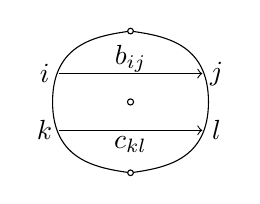
\begin{tikzpicture}[baseline=0,scale=0.6]
  \draw (-1.65,0) .. controls (-1.65,1.25) and (-0.7,1.4) .. (0,1.5);
  \draw (0,1.5) .. controls (0.7,1.4) and (1.65,1.25) .. (1.65,0);
  \draw (-1.65,0) .. controls (-1.65,-1.25) and (-0.7,-1.4) .. (0,-1.5);
  \draw (0,-1.5) .. controls (0.7,-1.4) and (1.65,-1.25) .. (1.65,0);
  \filldraw[fill=white] (0,1.5) circle (0.06);
  \filldraw[fill=white] (0,-1.5) circle (0.06);
  \filldraw[fill=white] (0,0) circle (0.065);
  \draw[->] (-1.52,0.6) -- (1.52,0.6);
  \draw[->] (-1.52,-0.6) -- (1.52,-0.6);
  \node at (-1.82,0.6) {$i$};
  \node at (1.82,0.6) {$j$};
  \node at (-1.82,-0.6) {$k$};
  \node at (1.82,-0.6) {$l$};
  \node at (0,0.91) {$b_{ij}$};
  \node at (0,-0.91) {$c_{kl}$};
\end{tikzpicture}
\]
The arc $b_{ij}$ cuts off a disk containing only the upper ideal
point, i.e.\ it is a \emph{corner arc} there, and $c_{kl}$ is a corner
arc at the lower ideal point. At the upper corner a rightward arc
is bad when its left state is smaller than its right state; at the
lower corner the inequality is reversed (the general rule is recalled
in (S4), Section~\ref{sec:statedskein}). Consequently, in the reduced
algebra,
\[
 b_{ij}=0\ (i<j),\qquad c_{kl}=0\ (k>l),
\]
so the matrix $B=(b_{ij})$ is lower triangular and $C=(c_{kl})$ is
upper triangular. If the intended diagram names the two arcs in the
opposite order, the two families must be renamed accordingly in all
formulas below.

\subsection{The main result and the structure of the proof}\label{sec:strategy}

Write $H^-_a$ and $H^+_a$ ($1\le a\le n$) for the two copies of the
toral generators $\hat K_a$ in $\U(\bm)$ and $\U(\bp)$, $E_i,F_i$
($1\le i<n$) for the Chevalley generators, and $s=q-q^{-1}$.
Informally, the answer to (1) is that the assignment
$b_{aa}\mapsto(H^-_a)^{-1}$, $c_{aa}\mapsto H^+_a$,
$b_{i+1,i}\mapsto -s\,F_i(H^-_{i+1})^{-1}$,
$c_{i,i+1}\mapsto s\,H^+_{i+1}E_i$
extends to an algebra isomorphism
$\Phi:\redS(\Bstar)\to\U(\bm)\bowtie\U(\bp)$, under which the remaining
arcs $b_{ji}$ and $c_{ij}$ with $j-i\ge2$ go to root vectors for the
roots $\pm(\epsilon_i-\epsilon_j)$ of $\slN$ times toral factors, and
the ideal $I$ goes to the ideal identifying the two tori, so that
$\redS(\Bstar)/I\cong\U(\slN)$. The precise statement, with all
conventions, is Theorem~\ref{thm:main}.
The proof has four inputs, assembled in Section~\ref{sec:proof}.
(i) \emph{A presentation of the double} (Proposition~\ref{prop:double}):
$\cD$ is generated by the two Borel algebras subject to explicit mixed
relations, so a homomorphism out of $\cD$ only has to be checked on
Chevalley generators.
(ii) \emph{A presentation of the skein algebra} (Lemma~\ref{lem:skein}):
$\redS(\Bstar)$ is generated by the entries of $B$ and $C$ subject to
the relations $RB_1B_2=B_2B_1R$, $RC_1C_2=C_2C_1R$, $RB_1C_2=C_2B_1R$
of $RTT$ type ($R$ the standard $R$-matrix, Section~\ref{sec:qmatrices})
and the triangularity and determinant conditions, and multiplication is a
linear isomorphism $A_\ell\ot A_u\cong\redS(\Bstar)$, where $A_\ell$,
$A_u$ are the triangular quantum matrix algebras
(Section~\ref{sec:qmatrices}). It is deduced from the L\^e--Sikora
factorization \cite{LS} of the \emph{unreduced} algebra by an explicit
computation showing that the bad-arc ideal is compatible with that
factorization.
(iii) \emph{Triangular quantum matrices are quantum Borel algebras}
(Lemma~\ref{lem:borel}), the Faddeev--Reshetikhin--Takhtajan realization
\cite{FRT} with precise normalizations; injectivity is proved by
comparing Poincar\'e--Birkhoff--Witt (PBW) bases, i.e.\ bases of
ordered monomials, on the two sides.
(iv) \emph{Verification of the mixed relations} in $\redS(\Bstar)$, a
short computation with the entries of $R$ (Section~\ref{sec:proof},
Steps 2--3).
We in fact construct $\Psi=\Phi^{-1}$ first, since (i) reduces its
existence to finitely many relations; bijectivity then follows from
the three established linear isomorphisms, because $\Psi$ is, on
underlying vector spaces, the composite of the triangular
decompositions $\cD\cong\U(\bm)\ot\U(\bp)\cong
A_\ell\ot A_u\cong\redS(\Bstar)$. The formulas for $\Phi$ on all arcs
follow by a recursion inside the triangular matrices, and part (2) is a
direct consequence (Section~\ref{sec:quotient}).

\subsection{Relation to the literature}

For $n=2$ the content of Theorem~\ref{thm:main} is known: Korinman
\cite[Theorems 1.2 and 2.20]{Ko} identifies the reduced stated
$SL_2$-skein algebra of the punctured bigon with the Drinfeld double of
the quantum Borel algebra, as a Hopf algebra, and obtains the
simply-connected quantum $\mathfrak{sl}_2$ as the quotient by
$K^{1/2}L^{1/2}-1$ (in Korinman's notation for the two toral
generators), our relation $b_{aa}c_{aa}=1$. A diagrammatic
precursor is Bigelow's definition of $\U(\mathfrak{sl}_2)$ \cite{Big};
the unreduced punctured bigon and its exchange relations are treated
for $SL_2$ in \cite[Section 4.8]{CL}, where the
factorization-and-exchange architecture used below originates. We are
not aware of a published statement of Theorem~\ref{thm:main} for
general $n$ (L\^e and Yu \cite[Section 1.9]{LY} announce related work of
L\^e and Sikora on the punctured bigon); it is an explicit higher-rank
version of an established rank-one identification, assembled from
standard ingredients cited where they are used. The reduction argument
in Lemma~\ref{lem:skein} is the punctured-bigon case of the mechanism
of \cite[Theorem 7.2]{LY}, made explicit.

\subsection{Conventions}\label{sec:conventions}

Throughout, $n\ge2$ and $\kk=\mathbb Q(q^{1/(2n)})$ with $q$ an
indeterminate; all algebras are unital associative $\kk$-algebras,
$\ot=\ot_\kk$, and $[x,y]=xy-yx$. We abbreviate $s=q-q^{-1}$, which is
invertible, as the pairing \eqref{eq:problempairing} requires.
Quantum groups are the unrestricted, simply-connected ones over $\kk$.
We write $\mathbf 1_{i<j}$, $\mathbf 1_{i>k}$, etc.\ for the truth
value ($0$ or $1$) of the indicated condition on indices, and
$\delta_{ij}$ for the Kronecker delta. Indices $a,b$, and all matrix and
state indices, run over $\{1,\dots,n\}$; the index $i$ of a Chevalley
generator $E_i,F_i$ (and of the $K_i$ of Section~\ref{sec:double}) runs
over $\{1,\dots,n-1\}$; root vectors and
off-diagonal matrix entries are indexed by pairs $1\le i<j\le n$.

\section{Borel algebras, the skew pairing and the double}\label{sec:double}

This section fixes the quantum-group side. We recall the
simply-connected Borel algebras, the Hopf structures and skew pairing
that enter the problem, and the generalized quantum double; we then
derive a presentation of the double (Proposition~\ref{prop:double}) and
state the main theorem.

\subsection{The simply-connected Borel algebras}

Put
\[
 \eta_{ai}=\delta_{ai}-\delta_{a,i+1}
 \qquad(1\le a\le n,\ 1\le i<n),
\]
so that $(\eta_{1i},\dots,\eta_{ni})$ is the coordinate vector of the
simple root $\alpha_i=\epsilon_i-\epsilon_{i+1}$ of $\slN$, where
$\epsilon_1,\dots,\epsilon_n$ are the coordinate functionals on the
diagonal matrices. The
\emph{positive Borel algebra} $\U(\bp)$ is the algebra generated by
$(H^+_a)^{\pm1}$ ($1\le a\le n$) and $E_i$ ($1\le i<n$) subject to
\begin{align}
 &H^+_aH^+_b=H^+_bH^+_a,\qquad \textstyle\prod_{a=1}^nH^+_a=1,
 \label{eq:torus}\\
 &H^+_aE_i(H^+_a)^{-1}=q^{\eta_{ai}}E_i, \label{eq:chevalley}\\
 &E_iE_j=E_jE_i\ \ (|i-j|>1),\qquad
 E_i^2E_j-(q+q^{-1})E_iE_jE_i+E_jE_i^2=0\ \ (|i-j|=1).
 \label{eq:serre}
\end{align}
The \emph{negative Borel algebra} $\U(\bm)$ is generated by
$(H^-_a)^{\pm1}$ and $F_i$ subject to \eqref{eq:torus} for the $H^-_a$,
to
\begin{equation}\label{eq:chevalleyminus}
 H^-_aF_i(H^-_a)^{-1}=q^{-\eta_{ai}}F_i,
\end{equation}
and to the Serre relations \eqref{eq:serre} with $E$ replaced by $F$.
We write $K^\pm_i=H^\pm_i(H^\pm_{i+1})^{-1}$, so that
$K^+_iE_j(K^+_i)^{-1}=q^{a_{ij}}E_j$ and
$K^-_iF_j(K^-_i)^{-1}=q^{-a_{ij}}F_j$ with $(a_{ij})$ the Cartan matrix
of $\slN$. The subalgebra
generated by the $H^\pm_a$ is the group algebra of
$\mathbb Z^n/\mathbb Z(1,\dots,1)$, the weight lattice of $\slN$
($H^\pm_a$ corresponding to the class of $\epsilon_a$), whereas the
adjoint version would contain only the root lattice spanned by the
$K^\pm_i$; this is what ``simply connected'' refers to.

The simply-connected quantum group $\U(\slN)$ is generated by
$H_a^{\pm1}$, $E_i$, $F_i$ subject to \eqref{eq:torus}, to
$H_aE_iH_a^{-1}=q^{\eta_{ai}}E_i$, $H_aF_iH_a^{-1}=q^{-\eta_{ai}}F_i$,
to the Serre relations for the $E_i$ and for the $F_i$, and to
\begin{equation}\label{eq:EFsl}
 [E_i,F_j]=\delta_{ij}\frac{K_i-K_i^{-1}}{s},\qquad K_i=H_iH_{i+1}^{-1}.
\end{equation}

\subsection{Hopf structure, skew pairing and the generalized double}

Both Borel algebras are Hopf algebras, with the $H^\pm_a$ group-like,
counit $\varepsilon(E_i)=\varepsilon(F_i)=0$, and (as in \cite[Chapter 6]{KS})
\begin{equation}\label{eq:coproduct}
 \Delta(E_i)=E_i\ot K^+_i+1\ot E_i,\qquad
 \Delta(F_i)=F_i\ot1+(K^-_i)^{-1}\ot F_i .
\end{equation}
We use Sweedler's notation $\Delta(a)=\sum a_{(1)}\ot a_{(2)}$. A
\emph{skew pairing} of $\U(\bp)$ with $\U(\bm)$ is a bilinear form
$\la\ ,\ \ra:\U(\bp)\times\U(\bm)\to\kk$ such that
$\la1,b\ra=\varepsilon(b)$, $\la a,1\ra=\varepsilon(a)$ and
\begin{equation}\label{eq:skew}
 \la aa',b\ra=\sum\la a,b_{(1)}\ra\la a',b_{(2)}\ra,\qquad
 \la a,bb'\ra=\sum\la a_{(1)},b'\ra\la a_{(2)},b\ra .
\end{equation}
By \eqref{eq:skew}, a skew pairing is determined by its values on pairs
of generators. The pairing in the problem is the
\emph{Drinfeld--Tanisaki pairing}
(\cite[Section 6.3.1]{KS}, \cite{Ta}; see also \cite[Section 13]{Dr}),
whose values on generators are, in our notation,
\begin{equation}\label{eq:pairing}
 \la H^+_a,H^-_b\ra=q^{1/n-\delta_{ab}},\qquad
 \la E_i,F_j\ra=-\frac{\delta_{ij}}s,\qquad
 \la H^+_a,F_i\ra=\la E_i,H^-_a\ra=0 .
\end{equation}
The exponent $\frac1n-\delta_{ab}$ is $-(\bar\epsilon_a,\bar\epsilon_b)$
for the invariant form on the weight lattice of $\slN$, $\bar\epsilon_a$
being the class of $\epsilon_a$. Two consequences of \eqref{eq:skew} for group-like
elements $H,H'$ will be used constantly: the pairing is multiplicative
in each group-like variable, and $\la H,(H')^{-1}\ra=\la H,H'\ra^{-1}$.

The \emph{generalized quantum double} (Drinfeld \cite[Section 13]{Dr};
\cite[Section 8.2.1]{KS}) of this skew-paired pair is the algebra
\[
 \cD=\U(\bm)\bowtie\U(\bp)
\]
whose underlying vector space is $\U(\bm)\ot\U(\bp)$, which contains
$\U(\bm)=\U(\bm)\ot1$ and $\U(\bp)=1\ot\U(\bp)$ as subalgebras, in which
$w\cdot u=w\ot u$ for $w\in\U(\bm)$, $u\in\U(\bp)$, and in which the
products in the other order are governed by the \emph{crossing rule}
\begin{equation}\label{eq:doublecross}
 \sum\la u_{(1)},w_{(1)}\ra\,u_{(2)}w_{(2)}
 =\sum\la u_{(2)},w_{(2)}\ra\,w_{(1)}u_{(1)}
 \qquad(u\in\U(\bp),\ w\in\U(\bm)).
\end{equation}
That these requirements define an associative algebra, in which the
multiplication map $\U(\bm)\ot\U(\bp)\to\cD$, $w\ot u\mapsto wu$, is a
linear isomorphism, is the basic theorem on the double
\cite[Section 8.2.1]{KS}; only its algebra structure is relevant here.
The form \eqref{eq:doublecross} of the crossing rule is the one of
\cite[Section 8.2.1]{KS} for a skew pairing satisfying \eqref{eq:skew};
as a consistency check, identifying the two tori in $\cD$ returns
$\U(\slN)$ with its standard relation \eqref{eq:EFsl}
(Section~\ref{sec:quotient}).

\subsection{A presentation of the double}

\begin{proposition}\label{prop:double}
The algebra $\cD$ is generated by $(H^\pm_a)^{\pm1}$, $E_i$, $F_i$
subject to the defining relations of $\U(\bp)$ and of $\U(\bm)$ together
with the mixed relations
\begin{align}
 H^-_aH^+_b&=H^+_bH^-_a, \label{eq:doubletorus}\\
 H^-_aE_i&=q^{\eta_{ai}}E_iH^-_a,
       & H^+_aF_i&=q^{-\eta_{ai}}F_iH^+_a, \label{eq:doubleweights}\\
 [E_i,F_j]&=\delta_{ij}\,\frac{K^+_i-(K^-_i)^{-1}}s. \label{eq:doubleEF}
\end{align}
\end{proposition}

\begin{proof}
\emph{The relations hold in $\cD$.} Apply \eqref{eq:doublecross} to
$u=E_i$, $w=F_j$. By \eqref{eq:coproduct}, the terms of the left side
are indexed by the four pairs of tensor factors; the pairings
$\la E_i,(K^-_j)^{-1}\ra$ and $\la1,F_j\ra=\varepsilon(F_j)$ vanish, while
$\la1,(K^-_j)^{-1}\ra=1$, so the left side is
$\la E_i,F_j\ra K^+_i+E_iF_j$. On the right side only
$\la K^+_i,1\ra F_jE_i$ and $\la E_i,F_j\ra(K^-_j)^{-1}$ survive.
Thus
$-\frac{\delta_{ij}}s K^+_i+E_iF_j=F_jE_i-\frac{\delta_{ij}}s(K^-_i)^{-1}$,
which is \eqref{eq:doubleEF}. For $u=H^+_a$, $w=F_i$ the rule reads
$\la H^+_a,(K^-_i)^{-1}\ra H^+_aF_i=F_iH^+_a$, and multiplicativity
gives
$\la H^+_a,(K^-_i)^{-1}\ra
 =\la H^+_a,H^-_i\ra^{-1}\la H^+_a,H^-_{i+1}\ra
 =q^{\delta_{ai}-\delta_{a,i+1}}=q^{\eta_{ai}}$,
which is the second relation in \eqref{eq:doubleweights}. For $u=E_i$,
$w=H^-_a$ the rule reads $E_iH^-_a=\la K^+_i,H^-_a\ra H^-_aE_i$ with
$\la K^+_i,H^-_a\ra=q^{-\eta_{ai}}$, which is the first relation. For
$u=H^+_b$, $w=H^-_a$ both sides carry the same nonzero scalar
$\la H^+_b,H^-_a\ra$, which cancels to give \eqref{eq:doubletorus}.

\emph{The relations are complete.} Let $P$ be the algebra presented by
the two Borel presentations and
\eqref{eq:doubletorus}--\eqref{eq:doubleEF}, and let $\pi:P\to\cD$ be
the canonical map; it is surjective because $\cD$ is generated by the
two Borel subalgebras. We claim that $P$ is spanned by the products
$wu$ with $w\in\U(\bm)$, $u\in\U(\bp)$. In a word in the generators,
call a pair consisting of a positive letter ($(H^+_a)^{\pm1}$, $E_i$)
and a negative letter ($(H^-_a)^{\pm1}$, $F_j$) standing anywhere to
its right an inversion. If a word has an inversion, it has one with the
two letters adjacent, and the mixed relations swap them: a toral swap
only introduces a scalar and lowers the number of inversions by one,
while \eqref{eq:doubleEF} replaces $E_iF_j$ by $F_jE_i$ (one inversion
fewer) plus a toral word with fewer Chevalley letters. By induction on
the number of Chevalley letters, and for a fixed number of them on the
number of inversions, every word becomes a linear combination of
products $wu$. Hence
$\mu:\U(\bm)\ot\U(\bp)\to P$, $w\ot u\mapsto wu$, is surjective, while
$\pi\circ\mu$ is the multiplication map of $\cD$, a linear isomorphism.
So $\mu$ is bijective, $\pi$ is injective, and $P\cong\cD$.
\end{proof}

\subsection{Root vectors and the main theorem}

For $1\le i<j\le n$ define root vectors recursively by
\begin{align}
 E_{i,i+1}&=E_i,&
 E_{ij}&=E_{i,j-1}E_{j-1}-q^{-1}E_{j-1}E_{i,j-1}
                  &&(j>i+1), \label{eq:Eroots}\\
 F_{i+1,i}&=F_i,&
 F_{ji}&=F_{j-1}F_{j-1,i}-qF_{j-1,i}F_{j-1}
                  &&(j>i+1). \label{eq:Froots}
\end{align}
Thus $E_{ij}$ has weight $\epsilon_i-\epsilon_j$ under both tori, i.e.\
$H^\pm_aE_{ij}(H^\pm_a)^{-1}=q^{\delta_{ai}-\delta_{aj}}E_{ij}$ by
\eqref{eq:chevalley} and \eqref{eq:doubleweights}, and $F_{ji}$ has
weight $\epsilon_j-\epsilon_i$. These normalizations make every
off-diagonal entry of $B$ and $C$ a single root vector times a toral
factor, with the uniform scalar $-s$, respectively $s$, independent of
$j-i$ (see \eqref{eq:rootmap}).

\begin{theorem}\label{thm:main}
Let $\redS(\Bstar)$ be the reduced stated $SL_n$-skein algebra of the
punctured bigon, with the arcs $b_{ij},c_{kl}$ of
Section~\ref{sec:interp}, and let $\cD=\U(\bm)\bowtie\U(\bp)$ be the
generalized quantum double of Section~\ref{sec:double}. An algebra
isomorphism $\Phi:\redS(\Bstar)\to\cD$ is given by
\begin{align}
 \Phi(b_{aa})&=(H^-_a)^{-1},&
 \Phi(c_{aa})&=H^+_a, \label{eq:diagonalmap}\\
 \Phi(b_{ji})&=-s\,F_{ji}(H^-_j)^{-1},&
 \Phi(c_{ij})&=s\,H^+_jE_{ij}
                       &&(i<j), \label{eq:rootmap}
\end{align}
the remaining entries being zero in $\redS(\Bstar)$: $b_{ij}=c_{ji}=0$
for $i<j$. Its inverse $\Psi$ is given on the generators of $\cD$ by
\begin{align}
 \Psi(H^-_a)&=b_{aa}^{-1},&
 \Psi(H^+_a)&=c_{aa}, \label{eq:inverseH}\\
 \Psi(F_i)&=-s^{-1}b_{i+1,i}\,b_{i+1,i+1}^{-1},&
 \Psi(E_i)&=s^{-1}c_{i+1,i+1}^{-1}\,c_{i,i+1}. \label{eq:inverseEF}
\end{align}
If $I\subset\redS(\Bstar)$ is the two-sided ideal generated by
$b_{aa}c_{aa}-1$, $1\le a\le n$, then $\Phi$ induces an isomorphism
\[
 \redS(\Bstar)/I\ \cong\ \U(\slN)
\]
with the simply-connected quantum group, under which $H_a$ (the
$\hat K_a$ of the problem), $E_i$, $F_i$ correspond to the classes of
$c_{aa}$ ($=b_{aa}^{-1}$ modulo $I$) and of the right-hand sides of
\eqref{eq:inverseEF}.
\end{theorem}

The diagonal entries $b_{aa}$, $c_{aa}$ are invertible in
$\redS(\Bstar)$ by Lemma~\ref{lem:skein} below, so the formulas make
sense.
The proof occupies Sections~\ref{sec:skein}--\ref{sec:quotient}, in the
order (ii), (iii), (iv), part (2) of Section~\ref{sec:strategy}.

\section{The reduced punctured bigon}\label{sec:skein}

\subsection{Stated skein algebras}\label{sec:statedskein}

We recall what is needed from \cite{LS,LY}. A punctured bordered
surface is $\mathfrak S=\overline{\mathfrak S}\setminus\mathcal P$,
where $\overline{\mathfrak S}$ is a compact oriented surface and
$\mathcal P$ is a finite set meeting every boundary component; the
points of $\mathcal P$ on the boundary are the \emph{ideal points},
those in the interior the \emph{punctures}, and the components of
$\partial\mathfrak S$ are the \emph{boundary edges}. Thus $\Bstar$ has
two ideal points, two boundary edges and one puncture. The stated $SL_n$-skein
algebra $\Skein(\mathfrak S)$ of \cite{LS} is the $\kk$-module spanned
by isotopy classes of \emph{stated $n$-webs} in
$\mathfrak S\times(-1,1)$, framed oriented tangles (more generally
webs) with endpoints on $\partial\mathfrak S\times(-1,1)$ carrying
\emph{states} in $\{1,\dots,n\}$, modulo the $SL_n$-skein relations of
\cite{LS}. The product $xy$ places $x$ above $y$, i.e.\ at
greater height in the $(-1,1)$ factor. Relative heights of endpoints on
the same boundary edge matter; for a single arc joining two different
boundary edges no such choice arises, so $b_{ij}$ and $c_{kl}$ are
determined by their isotopy class in $\Bstar$, their orientation and
their states. (The algebras of \cite{LS} are defined over any
commutative ring with an invertible $2n$-th root of $q$, and all
coefficients below lie in $\kk$; we work over $\kk$ throughout.)

We use the following four facts.

\noindent(S1) (\emph{Bigon} \cite[Theorem 6.3]{LS}; conventions as in
\cite[Sections 3.1 and 4.7]{LY}.) $\Skein(\Bigon)\cong\Oq$ as algebras,
the rightward arc with left state $i$ and right state $j$ corresponding
to the matrix generator $t_{ij}$; the matrix $T=(t_{ij})$ is a
$q$-matrix in the sense of Section~\ref{sec:qmatrices} below, with
quantum determinant $1$. The reversed arc is related to the antipode
by \cite[equation (83)]{LY}:
\begin{equation}\label{eq:antipode}
 S(t_{ij})=(-q)^{i-j}\,\overleftarrow{t}_{\,\bar j,\bar i},
 \qquad\bar i=n+1-i,
\end{equation}
where $\overleftarrow t_{kl}$ denotes the leftward arc with left state
$k$ and right state $l$. Only the fact that the scalar is nonzero will
matter.

\noindent(S2) (\emph{Factorization along saturated arcs}
\cite[Theorem 8.8, Corollaries 8.14--8.15]{LS}.) Let every component
of $\mathfrak S$ have nonempty boundary, and let
$\alpha_1,\dots,\alpha_m$ be a saturated system of disjoint proper arcs
in $\mathfrak S$ (each complementary region contains exactly one ideal
point or puncture, and the system is maximal with this property
\cite[Section 8.4]{LS}), each $\alpha_r$ joining two distinct boundary
edges. Then a thickening of each $\alpha_r$ is a bigon whose algebra
$A_{\alpha_r}\cong\Oq$ maps to $\Skein(\mathfrak S)$ by an algebra
homomorphism, and, for any fixed order of the factors, multiplication
$A_{\alpha_1}\ot\cdots\ot A_{\alpha_m}\to\Skein(\mathfrak S)$ is a
linear isomorphism. In general this is only a linear isomorphism; no
commutation between different factors is asserted.

\noindent(S3) (\emph{Height exchange} \cite[Section 4.10]{LY}.) A stated
web with two consecutive endpoints on the same boundary edge, both
oriented the same way (as for two rightward arcs), equals a linear
combination of the webs obtained by interchanging the heights of these
two endpoints, with the states permuted, the coefficients being entries
of the normalized matrix $q^{-1/n}R$, where $R$ is the matrix of
\eqref{eq:R} below (or entries of its inverse); they are computed from
the crossing evaluations \cite[equations (85)--(86)]{LY} and the counit
identity \cite[equation (90)]{LY}.

\noindent(S4) (\emph{Bad arcs and the reduced algebra}
\cite[Section 7.1]{LY}.) A corner arc at an ideal point $v$ is an arc
cutting off from $\mathfrak S$ a disk containing $v$ and no other ideal
point or puncture. Certain corner arcs, determined by the orientation
and an inequality between the two states, are \emph{bad}; for $\Bstar$
the rule is that a corner arc at the upper ideal point, of either
orientation, is bad when its state at the left endpoint is smaller than
its state at the right endpoint, and a corner arc at the lower ideal
point is bad when it is larger. The reduced algebra
$\redS(\mathfrak S)$ is the quotient of $\Skein(\mathfrak S)$ by the
two-sided ideal generated by all bad arcs.

\subsection{Quantum matrices}\label{sec:qmatrices}

Let $v_1,\dots,v_n$ be the standard basis of $\kk^n$, let $e_{ab}$ be
the matrix units of $\mathrm{End}(\kk^n)$, and put
\begin{equation}\label{eq:R}
 R=\sum_{a,b=1}^n q^{\delta_{ab}}e_{aa}\ot e_{bb}
       +s\sum_{a>b}e_{ab}\ot e_{ba},
 \qquad\text{so that}\qquad
 R(v_j\ot v_l)=q^{\delta_{jl}}v_j\ot v_l+s\,\mathbf1_{j<l}\,v_l\ot v_j.
\end{equation}
The $R$-matrix of the vector representation in the $SL_n$
normalization of \cite[Section 3.1]{LY} is $q^{-1/n}R$; the scalar
$q^{-1/n}$ does not affect the relations $RT_1T_2=T_2T_1R$ below and
is cancelled explicitly where it occurs (Step 2 of
Lemma~\ref{lem:skein}). We write $R^{ik}_{ab}$ for the entries of $R$,
$R(v_a\ot v_b)=\sum_{i,k}R^{ik}_{ab}\,v_i\ot v_k$. For a matrix $T$ with
entries in an algebra put $T_1=T\ot\id$ and $T_2=\id\ot T$. A
\emph{$q$-matrix} is a matrix $T$ with $RT_1T_2=T_2T_1R$
\cite{FRT}; in components (the entry in row $(i,k)$ and column $(j,l)$,
computed with \eqref{eq:R}),
\begin{equation}\label{eq:RTTcomponent}
 q^{\delta_{ik}}t_{ij}t_{kl}+s\mathbf1_{i>k}\,t_{kj}t_{il}
 =q^{\delta_{jl}}t_{kl}t_{ij}+s\mathbf1_{j<l}\,t_{kj}t_{il}.
\end{equation}
Equivalently, every $2\times2$ submatrix
$\left(\begin{smallmatrix}a&b\\c&d\end{smallmatrix}\right)$ satisfies
\begin{equation}\label{eq:qmatrix}
 ab=qba,\quad ac=qca,\quad bd=qdb,\quad cd=qdc,\quad
 bc=cb,\quad ad-da=sbc .
\end{equation}
The algebra $\Oq$ is generated by the entries of a universal $q$-matrix
with the relation $\det_qT=1$, where
$\det_qT=\sum_{\sigma\in S_n}(-q)^{\ell(\sigma)}t_{1\sigma(1)}\cdots
t_{n\sigma(n)}$, $\ell(\sigma)$ the number of inversions of $\sigma$
\cite[Section 9.2]{KS}.

Let $A_u$ (resp.\ $A_\ell$) be the \emph{universal upper} (resp.\
\emph{lower}) \emph{triangular $q$-matrix algebra}: it is generated by
$t_{ij}$ with $i\le j$ (resp.\ $i\ge j$), subject to the relations
\eqref{eq:qmatrix} of a $q$-matrix in which the other entries are set
to $0$, and to $\prod_at_{aa}=1$. We write $d_a=t_{aa}$. Three
consequences of \eqref{eq:qmatrix} will be used repeatedly.
(Q1) The $d_a$ commute: in the submatrix with rows and columns $i,k$
one off-diagonal entry is forbidden, so $ad-da=sbc$ reads
$d_id_k=d_kd_i$; as their product is $1$, each $d_a$ is invertible.
(Q2) In $A_u$ the relations \eqref{eq:qmatrix} give, for $i<j$, the
first formula below, and in $A_\ell$, for $i>j$, the second:
\begin{equation}\label{eq:toralmatrix}
 d_at_{ij}=q^{\delta_{ai}-\delta_{aj}}\,t_{ij}d_a\quad(i<j),\qquad
 d_at_{ij}=q^{\delta_{aj}-\delta_{ai}}\,t_{ij}d_a\quad(i>j).
\end{equation}
(Q3) For $i<k<j$, the $2\times2$ submatrices with rows $i,k$ and
columns $k,j$ in $A_u$, and with rows $k,j$ and columns $i,k$ in $A_\ell$,
give
\begin{equation}\label{eq:upperrec}
 [t_{ik},t_{kj}]=s\,t_{ij}d_k\quad\text{in }A_u,\qquad
 [t_{ki},t_{jk}]=s\,d_kt_{ji}\quad\text{in }A_\ell .
\end{equation}
Since $\det_q$ of a triangular matrix is the product of its diagonal
entries (only $\sigma=\id$ contributes), $A_u$ and $A_\ell$ are the
quotients of $\Oq$ by the strictly lower, respectively strictly upper,
entries. Transposition $t_{ij}\mapsto t_{ji}$ is an algebra isomorphism
$A_u\to A_\ell$, because \eqref{eq:qmatrix} is invariant under
$b\leftrightarrow c$.

\subsection{Presentation of \texorpdfstring{$\redS(\Bstar)$}{the reduced algebra}}

\begin{lemma}\label{lem:skein}
The algebra $\redS(\Bstar)$ is generated by the entries of
$B=(b_{ij})$ and $C=(c_{kl})$ subject to
\begin{gather}
 b_{ij}=0\ (i<j),\qquad c_{ij}=0\ (i>j),\qquad
 \prod_{a=1}^n b_{aa}=\prod_{a=1}^n c_{aa}=1, \label{eq:triangular}\\
 RB_1B_2=B_2B_1R,\qquad
 RC_1C_2=C_2C_1R,\qquad
 RB_1C_2=C_2B_1R. \label{eq:RTT}
\end{gather}
Moreover, the algebra homomorphisms $A_\ell\to\redS(\Bstar)$,
$f\mapsto f(B)$, and $A_u\to\redS(\Bstar)$, $g\mapsto g(C)$, obtained
by substituting $t_{ij}\mapsto b_{ij}$, respectively $t_{ij}\mapsto
c_{ij}$ (well defined because of
\eqref{eq:triangular}--\eqref{eq:RTT}), are injective, and the
multiplication map
\begin{equation}\label{eq:skeinfactor}
 A_\ell\ot A_u\longrightarrow\redS(\Bstar),\qquad
 f\ot g\longmapsto f(B)g(C),
\end{equation}
is a linear isomorphism. In particular the diagonal entries
$b_{aa}$, $c_{aa}$ are invertible in $\redS(\Bstar)$.
\end{lemma}

The $(i,k;j,l)$ component of the mixed relation $RB_1C_2=C_2B_1R$ is,
by \eqref{eq:RTTcomponent},
\begin{equation}\label{eq:mixedcomponent}
 q^{\delta_{ik}}b_{ij}c_{kl}+s\mathbf1_{i>k}\,b_{kj}c_{il}
 =q^{\delta_{jl}}c_{kl}b_{ij}+s\mathbf1_{j<l}\,c_{kj}b_{il}.
\end{equation}

\begin{proof}
\emph{Step 1: the unreduced factorization.}
A thin strip around either horizontal arc is a bigon, whose stated
skein algebra is $\Oq$ by (S1); write $A_B$ and $A_C$ for the two
copies, with generating matrices $B$ and $C$. Each arc joins the two
distinct boundary edges of $\Bstar$, so the inclusion of its strip
induces algebra homomorphisms $A_B\to\Skein(\Bstar)$ and
$A_C\to\Skein(\Bstar)$. The two arcs cut $\Bstar$ into two disks
containing one boundary ideal point each and a disk containing the
puncture, and any additional compact proper arc disjoint from these
arcs separates one of the complementary regions and leaves a component
containing neither a boundary ideal point nor an interior puncture.
Thus the system is saturated, and (S2) gives a linear isomorphism
\begin{equation}\label{eq:fullfactor}
 A_B\ot A_C\xrightarrow{\ \sim\ }\Skein(\Bstar),\qquad
 f\ot g\longmapsto f(B)g(C),\qquad A_B,A_C\cong\Oq .
\end{equation}

\emph{Step 2: the exchange relations.}
The first two relations in \eqref{eq:RTT} hold in $A_B$ and $A_C$ by
(S1). For the mixed relation, consider the two disjoint arcs with
states $(i,j)$ (upper arc) and $(k,l)$ (lower arc) placed so that the
$c$-end is higher at the left edge and the $b$-end is higher at the
right edge; this configuration is neither of the products
$b_{ij}c_{kl}$, $c_{kl}b_{ij}$. Applying (S3) at the left edge puts
the $b$-end on top there and expresses the configuration as a
combination of products $b_{pj}c_{rl}$ with coefficients
$q^{-1/n}R^{ik}_{pr}$; applying (S3) at the right edge instead puts the
$c$-end on top there and expresses it as a combination of products
$c_{kr}b_{ip}$ with coefficients $q^{-1/n}R^{pr}_{jl}$. By
\eqref{eq:R}, apart from the common factor $q^{-1/n}$, the identity
contribution has coefficient $q^{\delta_{ik}}$, respectively
$q^{\delta_{jl}}$, and the only other contribution is the interchange
of the two states, with coefficient $s$, which occurs when $i>k$,
respectively $j<l$. Equating the two expressions and cancelling
$q^{-1/n}$ gives exactly \eqref{eq:mixedcomponent}, i.e.\
$RB_1C_2=C_2B_1R$. That the exchange coefficients are entries of
$q^{-1/n}R$ rather than of its inverse is determined by the orientation
and height conventions of \cite[Section 4.10]{LY}; the quotient
computation of Section~\ref{sec:quotient} is consistent with this
choice but does not establish it.
\review{It would be helpful to include a picture here to accompany the text description.}
\emph{Step 3: the ideal of rightward bad arcs.}
Let $J_B\subset A_B$ be the two-sided ideal generated by the $b_{ij}$
with $i<j$ and $J_C\subset A_C$ the one generated by the $c_{kl}$ with
$k>l$; their generators are the rightward bad arcs. Under
\eqref{eq:fullfactor} consider the subspace
$N=J_B\ot A_C+A_B\ot J_C\subset\Skein(\Bstar)$. We claim that $N$ is the two-sided ideal generated by the rightward
bad arcs. Solving \eqref{eq:mixedcomponent} for the out-of-order
product, i.e.\ writing $C_2B_1=RB_1C_2R^{-1}$ with
$R^{-1}=\sum_{a,b}q^{-\delta_{ab}}e_{aa}\ot e_{bb}
-s\sum_{a>b}e_{ab}\ot e_{ba}$, gives
\begin{align}
 c_{kl}b_{ij}
 ={}&q^{\delta_{ik}-\delta_{jl}}\,b_{ij}c_{kl}
     +s\mathbf1_{i>k}\,q^{-\delta_{jl}}\,b_{kj}c_{il} \notag\\
   &-s\mathbf1_{j<l}\,q^{\delta_{ik}}\,b_{il}c_{kj}
     -s^2\mathbf1_{i>k}\mathbf1_{j<l}\,b_{kl}c_{ij}.
                                                        \label{eq:reorder}
\end{align}
In every term on the right, the $B$-entry has row index $\le i$ and
column index $\ge j$. Hence if $b_{ij}$ is bad ($i<j$), so is the $B$-entry of
every term; likewise the $C$-entry has row $\ge k$ and column $\le l$,
so a bad $C$-entry stays bad. Hence if a word in the entries of $B$
and $C$ contains a bad entry and is reordered into the form (word in
$B$)(word in $C$) by repeated use of \eqref{eq:reorder}, every summand
of the result still contains a bad entry of the same family. Since $J_B$, $J_C$ are ideals in their
own factors, this gives $N\cdot A_B\subset N$ and $A_C\cdot N\subset N$,
while $A_B\cdot N\subset N$ and $N\cdot A_C\subset N$ are clear. So $N$
is a two-sided ideal containing the rightward bad arcs and contained in
the ideal they generate, which proves the claim.

\emph{Step 4: the reversed bad arcs give nothing new.}
The bad arcs of the other orientation are the leftward corner arcs
$\overleftarrow b_{kl}$ with $k<l$ at the upper corner and
$\overleftarrow c_{kl}$ with $k>l$ at the lower one (in the notation
of (S1), applied in the strips $A_B$ and $A_C$). By
\eqref{eq:antipode} in $A_B$,
$\overleftarrow b_{kl}$ is a nonzero scalar multiple of
$S(b_{\bar l,\bar k})$, the $(\bar l,\bar k)$ entry of the inverse
matrix $B^{-1}$, and $k<l$ means $\bar l<\bar k$. In
$A_B/J_B\cong A_\ell$ (Section~\ref{sec:qmatrices}) the matrix $B$ is
lower triangular with invertible diagonal entries (Q1), hence has a
lower triangular inverse (write $B=D(1+D^{-1}L)$ with $D$ the diagonal
part of $B$ and $D^{-1}L$ strictly lower triangular, hence nilpotent).
Thus the strictly
upper entries of $B^{-1}$ vanish modulo $J_B$, and every
$\overleftarrow b_{kl}$ with $k<l$ lies in $J_B$. The same argument
applies to $\overleftarrow c_{kl}$, $k>l$, since
$(k,l)\mapsto(\bar l,\bar k)$ preserves both strict inequalities. Hence
$N$ is the full bad-arc ideal and $\redS(\Bstar)=\Skein(\Bstar)/N$.

\emph{Step 5: conclusion.}
By Section~\ref{sec:qmatrices}, $A_B/J_B\cong A_\ell$ and
$A_C/J_C\cong A_u$. Passing to the quotient by $N$ in
\eqref{eq:fullfactor}, and using
$(V\ot W)/(V'\ot W+V\ot W')\cong V/V'\ot W/W'$, gives the linear
isomorphism \eqref{eq:skeinfactor}; its restrictions to
$A_\ell\ot1$ and $1\ot A_u$ are the algebra homomorphisms
$f\mapsto f(B)$ and $g\mapsto g(C)$, which are therefore injective.
Finally, let $P$ be the algebra presented by
\eqref{eq:triangular}--\eqref{eq:RTT}. The relations hold in
$\redS(\Bstar)$, so there is a canonical surjection $P\to\redS(\Bstar)$;
by \eqref{eq:reorder} every word in $P$ is a combination of products
(word in $B$)(word in $C$), so $A_\ell\ot A_u\to P$ is surjective, and
its composite with $P\to\redS(\Bstar)$ is the bijection
\eqref{eq:skeinfactor}. As in the proof of
Proposition~\ref{prop:double}, $P\to\redS(\Bstar)$ is injective, and
the presentation is complete.
\end{proof}

\section{Triangular quantum matrices and the Borel algebras}\label{sec:borel}

That the upper and lower triangular quantum matrices realize the two
quantum Borel algebras is due to Faddeev, Reshetikhin and Takhtajan
\cite{FRT} (see also \cite[Section 8.5]{KS}). Since
Theorem~\ref{thm:main} is about precise normalizations, including the
order of the toral factors, we record the isomorphisms with proof;
$A_u$, $A_\ell$ and $d_a=t_{aa}$ are as in Section~\ref{sec:qmatrices}.

\begin{lemma}\label{lem:borel}
There are algebra isomorphisms
\begin{align}
 \U(\bp)&\xrightarrow{\ \sim\ }A_u,&
 H^+_a&\longmapsto d_a,&
 E_i&\longmapsto X_i:=s^{-1}d_{i+1}^{-1}t_{i,i+1}, \label{eq:upperborel}\\
 \U(\bm)&\xrightarrow{\ \sim\ }A_\ell,&
 H^-_a&\longmapsto d_a^{-1},&
 F_i&\longmapsto -s^{-1}t_{i+1,i}\,d_{i+1}^{-1}. \label{eq:lowerborel}
\end{align}
Under \eqref{eq:upperborel} the root vectors \eqref{eq:Eroots} map to
\begin{equation}\label{eq:rootimageborel}
 E_{ij}\longmapsto s^{-1}d_j^{-1}t_{ij}\qquad(i<j).
\end{equation}
\end{lemma}

\begin{proof}
\emph{The map \eqref{eq:upperborel} is a homomorphism.} The relations
\eqref{eq:torus} hold for the $d_a$ by (Q1), and \eqref{eq:chevalley}
follows from \eqref{eq:toralmatrix}: $d_a$ commutes with $d_{i+1}^{-1}$
and $d_at_{i,i+1}d_a^{-1}=q^{\delta_{ai}-\delta_{a,i+1}}t_{i,i+1}$.
For $|i-j|>1$ the elements $X_i,X_j$ commute: the diagonal factors
commute with one another, each diagonal factor commutes with the
off-diagonal entry occurring in the other $X$ by \eqref{eq:toralmatrix},
and $t_{i,i+1}$, $t_{j,j+1}$ lie in distinct rows and columns, so
\eqref{eq:qmatrix} gives $[t_{i,i+1},t_{j,j+1}]=s\,t_{i,j+1}t_{j,i+1}$
(for $i<j$), where $t_{j,i+1}=0$ because $j>i+1$. For the adjacent
Serre relations put $W_i=s^{-1}d_{i+2}^{-1}t_{i,i+2}$. Then
\begin{equation}\label{eq:Serrecheck}
 X_iX_{i+1}-q^{-1}X_{i+1}X_i=W_i,\qquad
 X_iW_i=qW_iX_i,\qquad W_iX_{i+1}=qX_{i+1}W_i.
\end{equation}
For the first identity, move the toral factors to the left using
\eqref{eq:toralmatrix} ($d_{i+2}$ commutes with $t_{i,i+1}$, and
$t_{i+1,i+2}d_{i+1}^{-1}=q\,d_{i+1}^{-1}t_{i+1,i+2}$), which turns the
left side into
$s^{-2}d_{i+1}^{-1}d_{i+2}^{-1}[t_{i,i+1},t_{i+1,i+2}]
 =s^{-1}d_{i+1}^{-1}d_{i+2}^{-1}\,t_{i,i+2}d_{i+1}
 =s^{-1}d_{i+2}^{-1}t_{i,i+2}=W_i$
by \eqref{eq:upperrec} and because $d_{i+1}$ commutes with
$t_{i,i+2}$. The other two identities reduce in the same way to the row
relation $t_{i,i+1}t_{i,i+2}=qt_{i,i+2}t_{i,i+1}$ and the column
relation $t_{i,i+2}t_{i+1,i+2}=qt_{i+1,i+2}t_{i,i+2}$. Substituting the
first identity of \eqref{eq:Serrecheck} into the second and third and
expanding yields
$X_i^2X_{i+1}-(q+q^{-1})X_iX_{i+1}X_i+X_{i+1}X_i^2=0$
and the same relation with $i$ and $i+1$ interchanged, i.e.\ both
adjacent Serre relations \eqref{eq:serre}. Thus \eqref{eq:upperborel}
defines a homomorphism $\phi:\U(\bp)\to A_u$.

\emph{Surjectivity and the root vectors.} By \eqref{eq:upperrec},
$t_{ij}=s^{-1}[t_{i,j-1},t_{j-1,j}]d_{j-1}^{-1}$ for $j>i+1$, so the
diagonal and first superdiagonal entries generate $A_u$ and $\phi$ is
surjective. The computation just made for the first identity in
\eqref{eq:Serrecheck}, with $(i,i+1,i+2)$ replaced by $(i,j-1,j)$ and
with the inductive hypothesis $\phi(E_{i,j-1})=s^{-1}d_{j-1}^{-1}t_{i,j-1}$,
gives \eqref{eq:rootimageborel}.

\emph{Injectivity, via PBW bases.} Order the pairs $i<j$
lexicographically. On the matrix side, the ordered monomials
\begin{equation}\label{eq:matrixPBW}
 \Bigl(\prod_{i<j}^{\mathrm{lex}}t_{ij}^{m_{ij}}\Bigr)
 d_1^{r_1}\cdots d_{n-1}^{r_{n-1}},
 \qquad m_{ij}\in\mathbb Z_{\ge0},\quad r_a\in\mathbb Z,
\end{equation}
form a basis of $A_u$. This follows from \cite[Proposition 3.10]{LY},
which gives such a basis, for any linear order of the off-diagonal
entries, for the lower triangular quotient, by transposition; there the
diagonal exponents are classes modulo $(1,\dots,1)$, uniquely
represented by $(r_1,\dots,r_{n-1},0)$, and since the $d_a$ are
invertible all integer exponents occur.
On the quantum-group side, the monomials
$\prod^{\mathrm{lex}}_{i<j}E_{ij}^{m_{ij}}$ form a basis of the
subalgebra $\U(\np)$ generated by the $E_i$ (PBW theorem in type $A$,
Rosso \cite{Ro}, Yamane \cite{Ya}). For the specific root vectors
\eqref{eq:Eroots} we use the Gr\"obner--Shirshov basis of
\cite[Theorem 3.1]{CSS} (going back to \cite{BM}), which by the
Composition--Diamond lemma \cite[Lemma 2.4]{CSS} yields exactly the
lexicographically ordered root monomials: in their $U_q(A_{n-1})$,
writing the quantum parameter as $v$, put $v=q^{1/2}$; their positive
Serre coefficient $v^2+v^{-2}$ becomes $q+q^{-1}$, and their recursion
$x_{ij}=v\,x_{i,j-1}E_{j-1}-v^{-1}E_{j-1}x_{i,j-1}$ gives
$x_{ij}=v^{j-i-1}E_{ij}$ by induction, so the basis assertion is
unchanged by this rescaling. Next, the torus acts on $\U(\np)$ by the
algebra automorphisms \eqref{eq:chevalley}: the Serre relations are
homogeneous, and the action descends to
$\mathbb Z^n/\mathbb Z(1,\dots,1)$ because $\sum_a\eta_{ai}=0$. Hence
$\U(\bp)$ is the smash product of $\U(\np)$ with the group algebra of
$\mathbb Z^n/\mathbb Z(1,\dots,1)$, and
\begin{equation}\label{eq:groupPBW}
 \Bigl(\prod_{i<j}^{\mathrm{lex}}E_{ij}^{m_{ij}}\Bigr)
 (H^+_1)^{r_1}\cdots(H^+_{n-1})^{r_{n-1}},
 \qquad m_{ij}\in\mathbb Z_{\ge0},\quad r_a\in\mathbb Z,
\end{equation}
is a basis of $\U(\bp)$.

Now apply $\phi$ to \eqref{eq:groupPBW}. By
\eqref{eq:rootimageborel} the image is
$\prod^{\mathrm{lex}}(s^{-1}d_j^{-1}t_{ij})^{m_{ij}}\cdot\prod_a d_a^{r_a}$.
Moving all diagonal factors to the right using \eqref{eq:toralmatrix}
only produces a nonzero scalar, and the exponent of $d_a$ becomes
$r_a-M_a$, where $M_a=\sum_{i<a}m_{ia}$ (so $M_1=0$); finally
$d_n^{-M_n}=(d_1\cdots d_{n-1})^{M_n}$. So the image is a nonzero
scalar times the basis monomial \eqref{eq:matrixPBW} with the same
$(m_{ij})$ and with $r_a$ replaced by $r_a-M_a+M_n$ for $a<n$. For
fixed $(m_{ij})$ this is a bijection of $\mathbb Z^{n-1}$. Distinct
basis elements therefore map to distinct basis elements, and $\phi$ is
injective.

\emph{The lower triangular case.} The assignment
$H^-_a\mapsto(H^+_a)^{-1}$, $F_i\mapsto-q^{-1}E_i$
is an algebra isomorphism $\U(\bm)\to\U(\bp)$: it carries
\eqref{eq:chevalleyminus} to \eqref{eq:chevalley}, and the Serre
relations are homogeneous (any nonzero scalar in place of $-q^{-1}$
would do; this one makes the composite below come out as
\eqref{eq:lowerborel}). Composing it with \eqref{eq:upperborel} and
with transposition $A_u\to A_\ell$ (Section~\ref{sec:qmatrices}) gives
an isomorphism $\U(\bm)\to A_\ell$ with $H^-_a\mapsto d_a^{-1}$ and
$F_i\mapsto-q^{-1}s^{-1}d_{i+1}^{-1}t_{i+1,i}$, which equals
$-s^{-1}t_{i+1,i}d_{i+1}^{-1}$ by \eqref{eq:toralmatrix} for $A_\ell$:
$d_{i+1}t_{i+1,i}=q^{-1}t_{i+1,i}d_{i+1}$. This is
\eqref{eq:lowerborel}.
\end{proof}

\section{Proof of Theorem \ref{thm:main}: the isomorphism}\label{sec:proof}

We construct $\Psi:\cD\to\redS(\Bstar)$ first, because
Proposition~\ref{prop:double} reduces its existence to finitely many
relations, and then obtain $\Phi$ as its inverse. In $\redS(\Bstar)$
abbreviate
\[
 d_a=b_{aa},\qquad h_a=c_{aa},\qquad
 x_i=b_{i+1,i},\qquad y_i=c_{i,i+1}
\]
(so the $d_a$ of Lemma~\ref{lem:borel} become $d_a$ when the lemma is
applied to $B$ and $h_a$ when it is applied to $C$).

\emph{Step 1: the two Borel algebras embed.} By Lemma~\ref{lem:skein},
$C$ is an upper triangular $q$-matrix with $\prod_ah_a=1$ and $B$ a
lower triangular one with $\prod_ad_a=1$, and $g\mapsto g(C)$,
$f\mapsto f(B)$ are injective algebra maps $A_u\to\redS(\Bstar)$,
$A_\ell\to\redS(\Bstar)$. Composing with Lemma~\ref{lem:borel} gives
injective algebra homomorphisms
\begin{gather*}
 \U(\bp)\to\redS(\Bstar):\quad H^+_a\mapsto h_a,\quad
 E_i\mapsto e_i:=s^{-1}h_{i+1}^{-1}y_i,\\
 \U(\bm)\to\redS(\Bstar):\quad H^-_a\mapsto d_a^{-1},\quad
 F_i\mapsto f_i:=-s^{-1}x_id_{i+1}^{-1}.
\end{gather*}
These are the assignments \eqref{eq:inverseH}--\eqref{eq:inverseEF}.
By Proposition~\ref{prop:double}, they define a homomorphism
$\Psi:\cD\to\redS(\Bstar)$ as soon as the mixed relations
\eqref{eq:doubletorus}--\eqref{eq:doubleEF} hold for
$d_a^{-1},h_a,e_i,f_i$.

\emph{Step 2: the mixed relations between the arcs.} Specializing
\eqref{eq:mixedcomponent} and using triangularity, we get
\begin{align}
 d_ah_b&=h_bd_a, \label{eq:arctorus}\\
 d_ay_i&=q^{-\eta_{ai}}y_id_a,&
 h_ax_i&=q^{-\eta_{ai}}x_ih_a, \label{eq:arcweights}\\
 x_jy_i&=q^{\delta_{j,i+1}-\delta_{j+1,i}}\,y_ix_j
                                                    &&(i\ne j), \label{eq:arcoff}\\
 [x_i,y_i]&=s\,(h_id_{i+1}-d_ih_{i+1}). \label{eq:arcsame}
\end{align}
Indeed, for $(i,k;j,l)=(a,r;a,r)$ the two $s$-terms of
\eqref{eq:mixedcomponent} contain $b_{ra}$ with $r<a$ or $c_{ra}$ with
$r>a$, which vanish, leaving \eqref{eq:arctorus}; in the same way
$(a,r;a,r+1)$ gives $q^{\delta_{ar}}d_ay_r=q^{\delta_{a,r+1}}y_rd_a$,
the first relation in \eqref{eq:arcweights}, and $(r+1,a;r,a)$ gives
the second. For $(i,k;j,l)=(t+1,r;t,r+1)$ the relation reads
$q^{\delta_{t+1,r}}x_ty_r+s\mathbf1_{t+1>r}\,b_{rt}c_{t+1,r+1}
 =q^{\delta_{t,r+1}}y_rx_t+s\mathbf1_{t<r+1}\,c_{rt}b_{t+1,r+1}$,
and by triangularity the $s$-terms vanish unless $r=t$. For $r\ne t$
this is \eqref{eq:arcoff} with $(i,j)=(r,t)$; for $r=t$ it reads
$x_ry_r+s\,d_rh_{r+1}=y_rx_r+s\,h_rd_{r+1}$, which is
\eqref{eq:arcsame}.

\emph{Step 3: the mixed relations of the double.} Relations
\eqref{eq:arctorus}--\eqref{eq:arcweights}, together with the fact
that $d_a$, $h_a$ commute with $d_b$, $h_b$, are exactly
\eqref{eq:doubletorus}--\eqref{eq:doubleweights} for $d_a^{-1}$, $h_a$,
$e_i$, $f_i$: for instance $d_a^{-1}e_i=q^{\eta_{ai}}e_id_a^{-1}$
because $d_a^{-1}$ commutes with $h_{i+1}^{-1}$ and
$d_a^{-1}y_i=q^{\eta_{ai}}y_id_a^{-1}$ by \eqref{eq:arcweights}. For
\eqref{eq:doubleEF} with $i\ne j$, rewrite
$e_if_j=-s^{-2}h_{i+1}^{-1}y_ix_jd_{j+1}^{-1}$ in the order
$x_jd_{j+1}^{-1}h_{i+1}^{-1}y_i$ of the factors of $f_je_i$; the three
moves
$y_ix_j\to x_jy_i$, $h_{i+1}^{-1}x_j\to x_jh_{i+1}^{-1}$,
$y_id_{j+1}^{-1}\to d_{j+1}^{-1}y_i$ contribute, by \eqref{eq:arcoff}
and \eqref{eq:arcweights}, the total exponent
$(\delta_{j+1,i}-\delta_{j,i+1})+\eta_{i+1,j}-\eta_{j+1,i}=0$,
so $e_if_j=f_je_i$. For $i=j$, the internal relation
\eqref{eq:toralmatrix} ($h_{i+1}^{-1}y_i=q\,y_ih_{i+1}^{-1}$) and the
mixed relations \eqref{eq:arcweights}
($d_{i+1}^{-1}y_i=q^{-1}y_id_{i+1}^{-1}$,
$h_{i+1}^{-1}x_i=q^{-1}x_ih_{i+1}^{-1}$) give, the powers of $q$
cancelling,
$e_if_i=-s^{-2}\,y_ix_i\,h_{i+1}^{-1}d_{i+1}^{-1}$ and
$f_ie_i=-s^{-2}\,x_iy_i\,h_{i+1}^{-1}d_{i+1}^{-1}$.
Hence, by \eqref{eq:arcsame},
\begin{equation}\label{eq:verifiedEF}
 [e_i,f_j]=\delta_{ij}\,s^{-2}[x_i,y_i]\,h_{i+1}^{-1}d_{i+1}^{-1}
 =\delta_{ij}\,\frac{h_ih_{i+1}^{-1}-d_id_{i+1}^{-1}}s
 =\Psi\Bigl(\delta_{ij}\frac{K^+_i-(K^-_i)^{-1}}s\Bigr),
\end{equation}
since $\Psi(K^+_i)=h_ih_{i+1}^{-1}$ and
$\Psi((K^-_i)^{-1})=d_{i+1}^{-1}d_i$. By Proposition~\ref{prop:double},
$\Psi:\cD\to\redS(\Bstar)$ is a well-defined algebra homomorphism.

\emph{Step 4: bijectivity.} On underlying vector spaces $\Psi$ is the
composite of three linear isomorphisms,
\begin{equation}\label{eq:bijective}
 \cD\ \xrightarrow{\ \sim\ }\ \U(\bm)\ot\U(\bp)
 \ \xrightarrow[\text{Lemma \ref{lem:borel}}]{\ \sim\ }\
 A_\ell\ot A_u
 \ \xrightarrow[\text{Lemma \ref{lem:skein}}]{\ \sim\ }\
 \redS(\Bstar),
\end{equation}
the first being the inverse of multiplication in the double and the
last the multiplication map \eqref{eq:skeinfactor}: indeed, by Step 1,
$\Psi$ restricted to $\U(\bm)$ is \eqref{eq:lowerborel} followed by
$f\mapsto f(B)$, and restricted to $\U(\bp)$ it is \eqref{eq:upperborel}
followed by $g\mapsto g(C)$, so
$\Psi(wu)=\Psi(w)\Psi(u)$ with $\Psi(w)$ in the image of $A_\ell$ and
$\Psi(u)$ in the image of $A_u$. Hence $\Psi$ is bijective and
$\Phi:=\Psi^{-1}$ is an algebra isomorphism satisfying
\eqref{eq:diagonalmap} and the case $j=i+1$ of \eqref{eq:rootmap}.

\emph{Step 5: the formula for $\Phi$ on all arcs.} It remains to check
\eqref{eq:rootmap} for $j>i+1$; the entries $b_{ij}$, $c_{ji}$ with
$i<j$ vanish by \eqref{eq:triangular}. By \eqref{eq:upperrec} applied to
$C$ and $B$, and since $h_k$ and $d_k$ commute with $c_{ij}$ and $b_{ji}$
for $i<k<j$,
\begin{equation}\label{eq:arcrec}
 c_{ij}=s^{-1}h_k^{-1}[c_{ik},c_{kj}],\qquad
 b_{ji}=s^{-1}d_k^{-1}[b_{ki},b_{jk}]\qquad(i<k<j).
\end{equation}
Take $k=j-1$ and argue by induction on $j-i$. In the first recurrence,
substituting $\Phi(c_{ik})=sH^+_kE_{ik}$ and
$\Phi(c_{kj})=sH^+_jE_{k}$ and moving the toral factors to the left
($H^+_j$ commutes with $E_{ik}$, and $E_kH^+_k=q^{-1}H^+_kE_k$) gives
$\Phi(c_{ij})=s\,(H^+_k)^{-1}H^+_kH^+_j
 \bigl(E_{ik}E_k-q^{-1}E_kE_{ik}\bigr)=s\,H^+_jE_{ij}$.
In the second, substituting $\Phi(b_{ki})=-sF_{ki}(H^-_k)^{-1}$ and
$\Phi(b_{jk})=-sF_k(H^-_j)^{-1}$, moving $(H^-_k)^{-1}$ past $F_k$
introduces a factor $q$ by \eqref{eq:chevalleyminus}, $(H^-_j)^{-1}$
commutes with $F_{ki}$, and $H^-_k$ commutes with $F_{ki}F_k$ and
$F_kF_{ki}$ (their weight is $\epsilon_j-\epsilon_i$, on which $H^-_k$
acts trivially), so that
\[
 \Phi(b_{ji})=s\bigl(qF_{ki}F_k-F_kF_{ki}\bigr)(H^-_j)^{-1}
 =-s\,F_{ji}(H^-_j)^{-1}
\]
by \eqref{eq:Froots}. This proves \eqref{eq:rootmap} and completes
part (1) of the theorem. \qed

\section{The diagonal quotient}\label{sec:quotient}

We now prove part (2). Under $\Phi$ the generators of $I$ become
\begin{equation}\label{eq:idealimage}
 b_{aa}c_{aa}-1\longmapsto(H^-_a)^{-1}H^+_a-1 .
\end{equation}
The elements $z_a=(H^-_a)^{-1}H^+_a$ are central in $\cD$: the two
tori commute, and by \eqref{eq:chevalley},
\eqref{eq:chevalleyminus} and \eqref{eq:doubleweights} the elements
$H^-_a$ and $H^+_a$ have the same conjugation action on every $E_i$ and
on every $F_i$. Since the $H^\pm_a$ are units, the ideal generated by
the $z_a-1$ is $\Phi(I)=J:=(H^+_a-H^-_a\mid1\le a\le n)$, so
$\redS(\Bstar)/I\cong\cD/J$. Recovering a
quantum group from the double of its Borel algebras by identifying the
two tori is the standard construction \cite[Section 13]{Dr},
\cite[Section 8.2.4]{KS}; we spell it out for the presentation in use. In $\cD/J$ write $H_a$ for the common image of
$H^\pm_a$ and $K_i=H_iH_{i+1}^{-1}$. The presentation of
Proposition~\ref{prop:double} becomes: the relations \eqref{eq:torus}
for the $H_a$, $H_aE_iH_a^{-1}=q^{\eta_{ai}}E_i$,
$H_aF_iH_a^{-1}=q^{-\eta_{ai}}F_i$, the Serre relations, and
$[E_i,F_j]=\delta_{ij}(K_i-K_i^{-1})/s$, while
\eqref{eq:doubletorus}--\eqref{eq:doubleweights} become redundant. This
is the presentation of the simply-connected $\U(\slN)$ given in
Section~\ref{sec:double}, so $\cD/J\cong\U(\slN)$ with
$H^\pm_a\mapsto H_a$, $E_i\mapsto E_i$, $F_i\mapsto F_i$.
Thus $\redS(\Bstar)/I\cong\cD/J\cong\U(\slN)$; composing with $\Psi$
and reading off \eqref{eq:inverseH}--\eqref{eq:inverseEF} modulo $I$
gives the explicit correspondences stated at the end of
Theorem~\ref{thm:main}. That the sign and toral factors of \eqref{eq:doubleEF}
reproduce the standard relation \eqref{eq:EFsl} is a consistency check
on the conventions of Section~\ref{sec:double}, not a derivation of
them. \qed

\begin{thebibliography}{99}

\bibitem{Big}
S.~Bigelow,
\emph{A diagrammatic definition of $U_q(\mathfrak{sl}_2)$},
J. Knot Theory Ramifications \textbf{23} (2014), no.~6, 1450036.

\bibitem{BM}
L.~A.~Bokut and P.~Malcolmson,
\emph{Gr\"obner--Shirshov bases for quantum enveloping algebras},
Israel J. Math. \textbf{96} (1996), 97--113.

\bibitem{CSS}
Y.~Chen, H.~Shao and K.~P.~Shum,
\emph{Rosso--Yamane theorem on PBW basis of $U_q(A_N)$},
CUBO \textbf{10} (2008), no.~3, 171--194; arXiv:0804.0954v1.

\bibitem{CL}
F.~Costantino and T.~T.~Q.~L\^e,
\emph{Stated skein algebras of surfaces},
J. Eur. Math. Soc. \textbf{24} (2022), no.~12, 4063--4142.

\bibitem{Dr}
V.~G.~Drinfeld,
\emph{Quantum groups},
Proceedings of the International Congress of Mathematicians (Berkeley,
1986), vol.~1, Amer. Math. Soc., 1987, 798--820.

\bibitem{FRT}
N.~Yu.~Reshetikhin, L.~A.~Takhtadzhyan and L.~D.~Faddeev,
\emph{Quantization of Lie groups and Lie algebras},
Leningrad Math. J. \textbf{1} (1990), no.~1, 193--225.

\bibitem{KS}
A.~Klimyk and K.~Schm\"udgen,
\emph{Quantum Groups and Their Representations},
Springer, Berlin, 1997.

\bibitem{Ko}
J.~Korinman,
\emph{Quantum holonomic link invariants derived from stated skein
algebras}, arXiv:1907.01732v4 (2024).

\bibitem{Le}
T.~T.~Q.~L\^e,
\emph{Triangular decomposition of skein algebras},
Quantum Topol. \textbf{9} (2018), no.~3, 591--632.

\bibitem{LS}
T.~T.~Q.~L\^e and A.~S.~Sikora,
\emph{Stated $SL(n)$-skein modules and algebras},
J. Topol. \textbf{17} (2024), no.~3, e12350; arXiv:2201.00045v3
(theorem numbers refer to this version).

\bibitem{LY}
T.~T.~Q.~L\^e and T.~Yu,
\emph{Quantum traces for $SL_n$-skein algebras},
arXiv:2303.08082v2 (2025) (theorem and equation numbers refer to this
version).

\bibitem{Ro}
M.~Rosso,
\emph{An analogue of P.B.W. theorem and the universal $R$-matrix for
$U_h\mathfrak{sl}(N+1)$},
Comm. Math. Phys. \textbf{124} (1989), no.~2, 307--318.

\bibitem{Ta}
T.~Tanisaki,
\emph{Killing forms, Harish-Chandra isomorphisms, and universal
$R$-matrices for quantum algebras},
Internat. J. Modern Phys. A \textbf{7}, Suppl. 1B (1992), 941--961.

\bibitem{Ya}
H.~Yamane,
\emph{A Poincar\'e--Birkhoff--Witt theorem for quantized universal
enveloping algebras of type $A_N$},
Publ. Res. Inst. Math. Sci. \textbf{25} (1989), no.~3, 503--520.

\end{thebibliography}

\end{document}
